\section{Experimentos e resultados}

Os experimentos finais utilizam as instâncias dos conjuntos A, B e F disponíveis no diretório \texttt{instancias}. O GRASP clássico foi configurado com $\alpha=0.25$, 50 iterações e 20 movimentos locais. O GRASP Reativo utilizou uma grade de $\alpha$ com passo $0.05$, bloco de atualização igual a 2 e $\delta=5$.

Os dois métodos foram executados cinco vezes em cada instância. Foram registrados custo mínimo, custo médio, tempo mínimo, tempo médio e gaps. A agregação apresentou gap mínimo médio de 14.79\% no clássico e 14.29\% no reativo; os gaps médios foram 17.63\% e 17.24\%. O tempo médio foi 4.23 s no clássico e 6.05 s no reativo.

Considerando as cinco execuções de cada uma das 50 instâncias, o tempo agregado aproximado foi de 1057.86 s (17 min 38 s) para o GRASP clássico e 1513.44 s (25 min 13 s) para o GRASP Reativo. Os resultados completos das cinco execuções de ambos os métodos estão disponíveis no \href{https://drive.google.com/drive/folders/1VtNmJa1JuUNSUU0BtCh_EowPccevDMAs?usp=sharing}{Drive\textsuperscript{2}}. O código, os experimentos e o notebook Jupyter estão disponíveis no \href{https://github.com/joaosoaressantos22/meta_heuristicas.git}{GitHub\textsuperscript{3}}.

\begin{table}[htbp]
\centering
\caption{Resultados finais das instâncias utilizadas na análise de convergência e TTT.}
\label{tab:destaques}
\small
\begin{tabular}{llrrrrr}
\toprule
Instância & Método & Ótimo & Mínimo & Médio & Gap mín. & Gap méd. \\
\midrule
A-n33-k5 & GRASP $\alpha=0.25$ & 661 & 670 & 687.2 & 1.36\% & 3.96\% \\
A-n33-k5 & Reactive GRASP & 661 & 669 & 677.6 & 1.21\% & 2.51\% \\
B-n31-k5 & GRASP $\alpha=0.25$ & 672 & 675 & 680.8 & 0.45\% & 1.31\% \\
B-n31-k5 & Reactive GRASP & 672 & 677 & 679.0 & 0.74\% & 1.04\% \\
\bottomrule
\end{tabular}
\end{table}

Em A-n33-k5, o reativo obteve melhor custo mínimo e médio. Em B-n31-k5, o clássico obteve melhor custo mínimo, mas o reativo obteve melhor custo médio.

\begin{figure}[htbp]
\centering
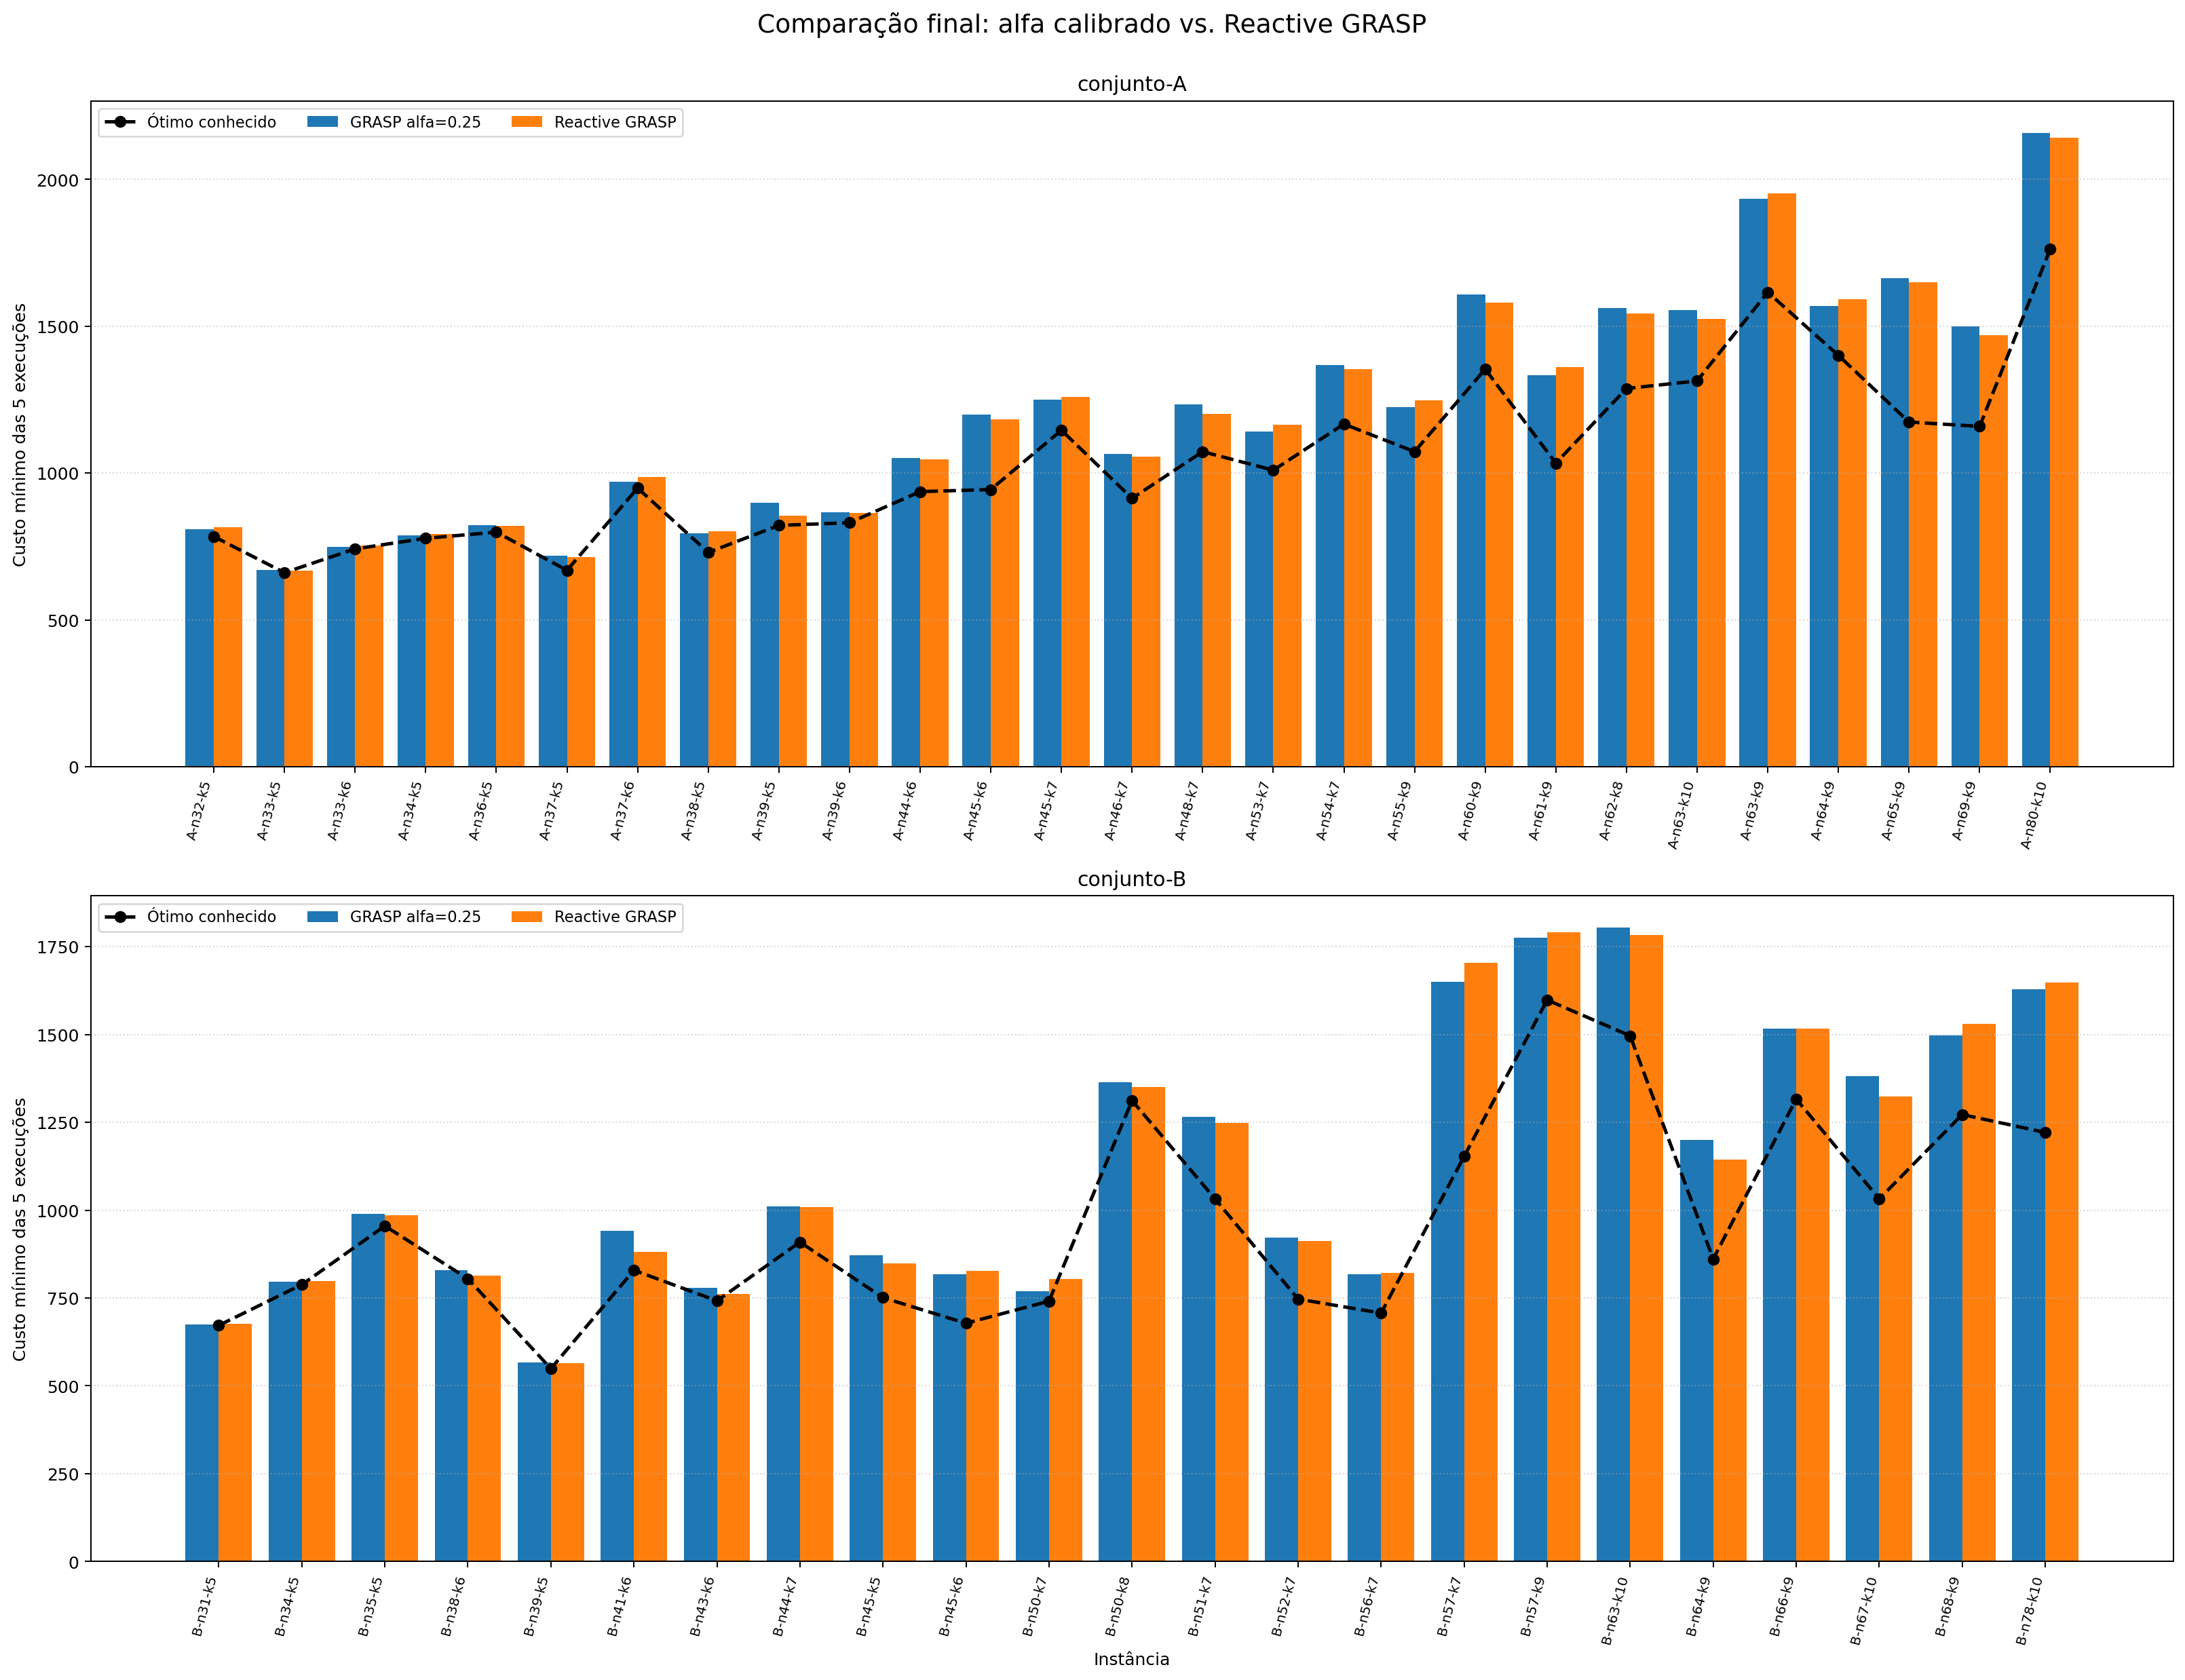
\includegraphics[width=0.90\textwidth]{imagens/comparacao_final_grasp.png}
\caption{Comparação dos custos mínimos do GRASP clássico calibrado e do GRASP Reativo.}
\label{fig:comparacao}
\end{figure}

Os gráficos de convergência mostram o melhor custo após cada solução construída e melhorada. O TTT considera o tempo até o primeiro registro igual ao ótimo conhecido; sua construção segue a abordagem de Aiex, Resende e Ribeiro \cite{aiex2007}.

\begin{figure}[htbp]
\centering
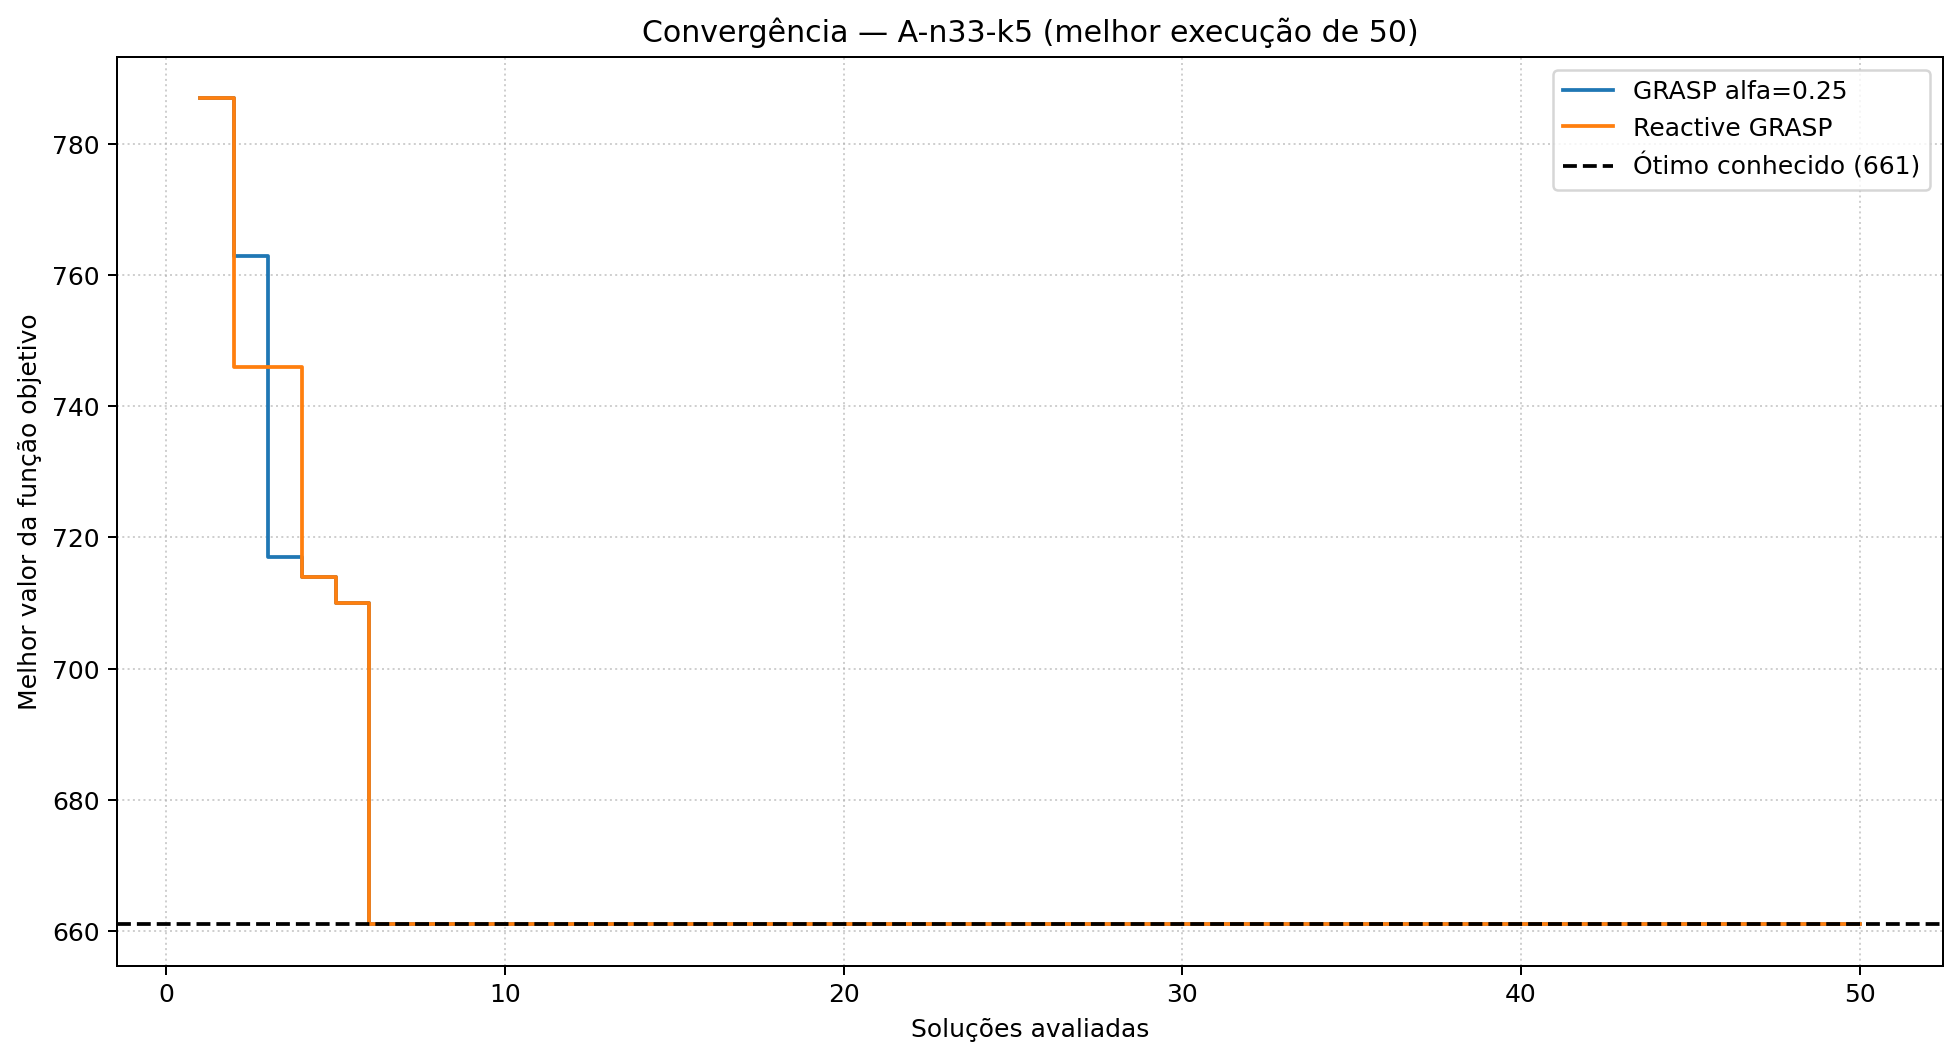
\includegraphics[width=0.98\textwidth]{imagens/convergencia_A-n33-k5.png}
\caption{Convergência em A-n33-k5.}
\label{fig:convergenciaA}
\end{figure}

\begin{figure}[htbp]
\centering
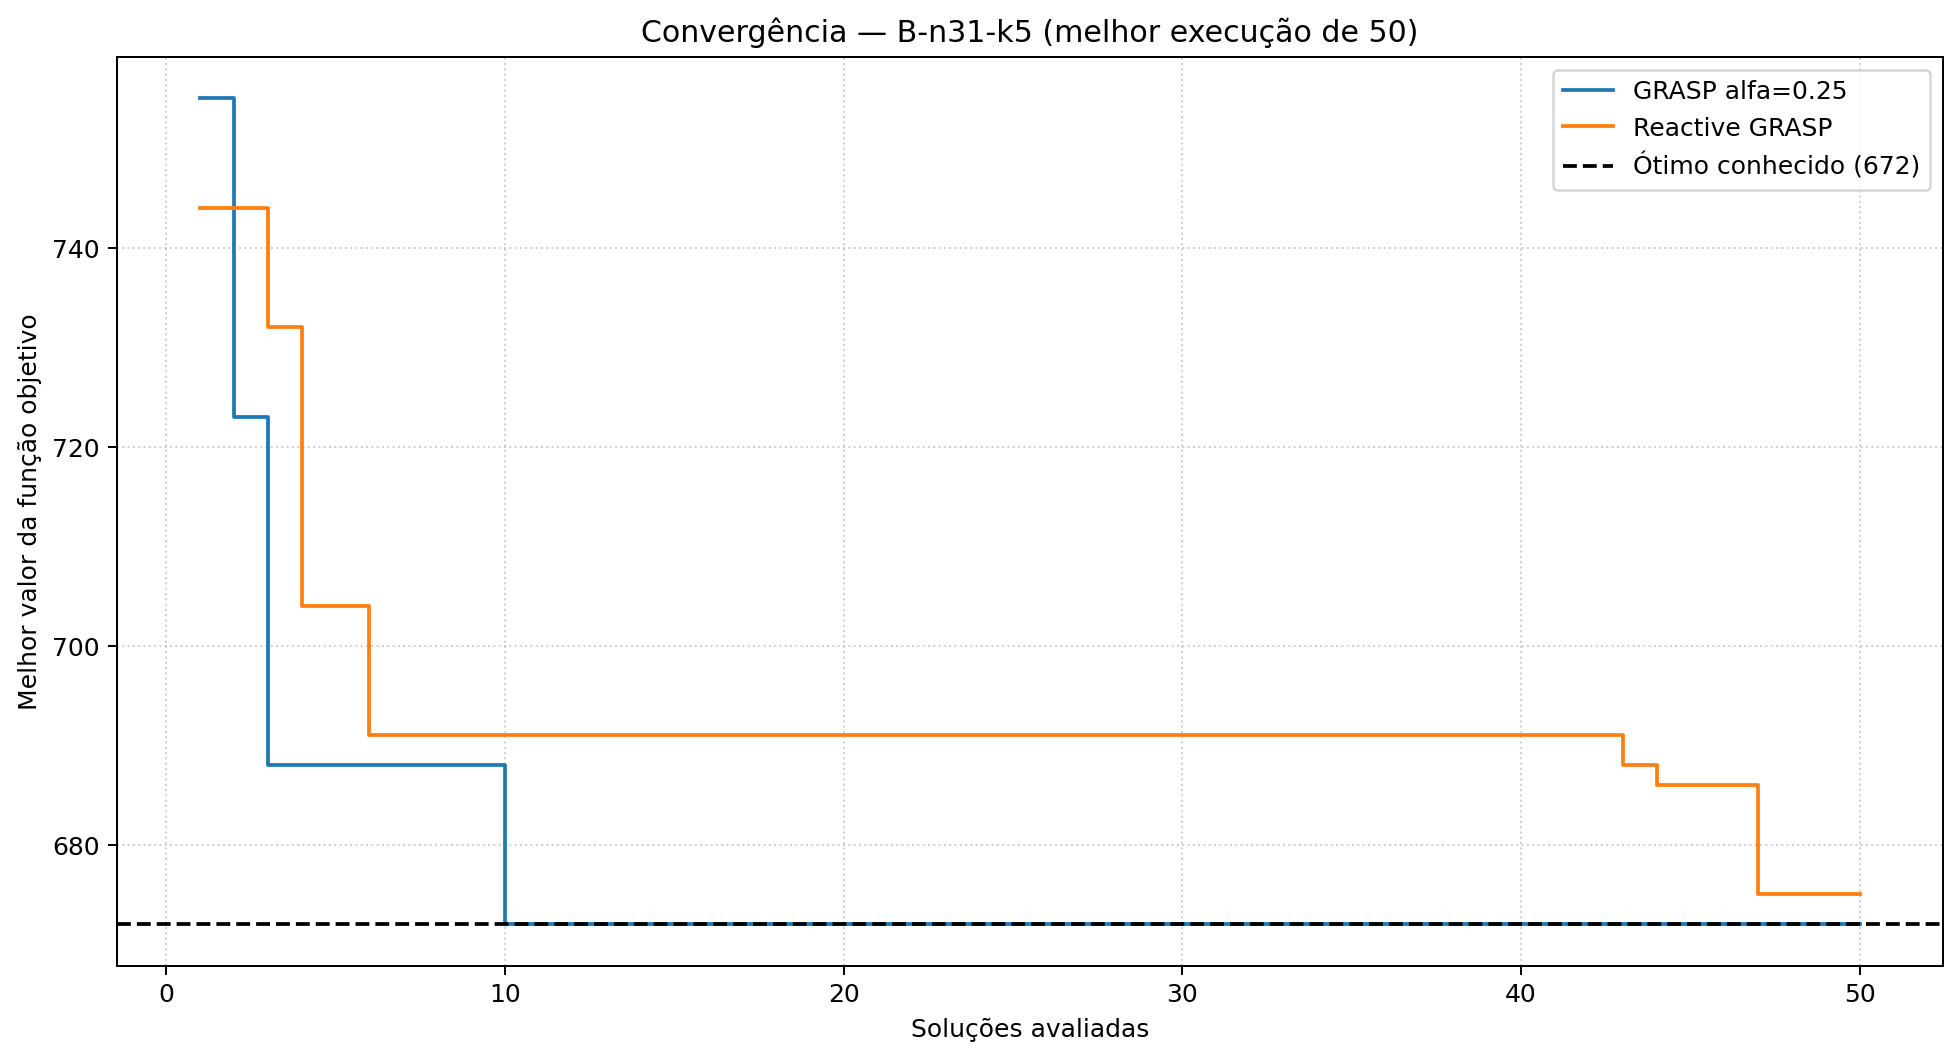
\includegraphics[width=0.98\textwidth]{imagens/convergencia_B-n31-k5.png}
\caption{Convergência em B-n31-k5.}
\label{fig:convergenciaB}
\end{figure}

Nas duas instâncias, o custo decresce rapidamente nas primeiras avaliações. Em A-n33-k5, o clássico atingiu o ótimo em duas das 50 execuções e o reativo em uma. Em B-n31-k5, o clássico encontrou o ótimo uma vez e o reativo nenhuma vez.

\begin{figure}[htbp]
\centering
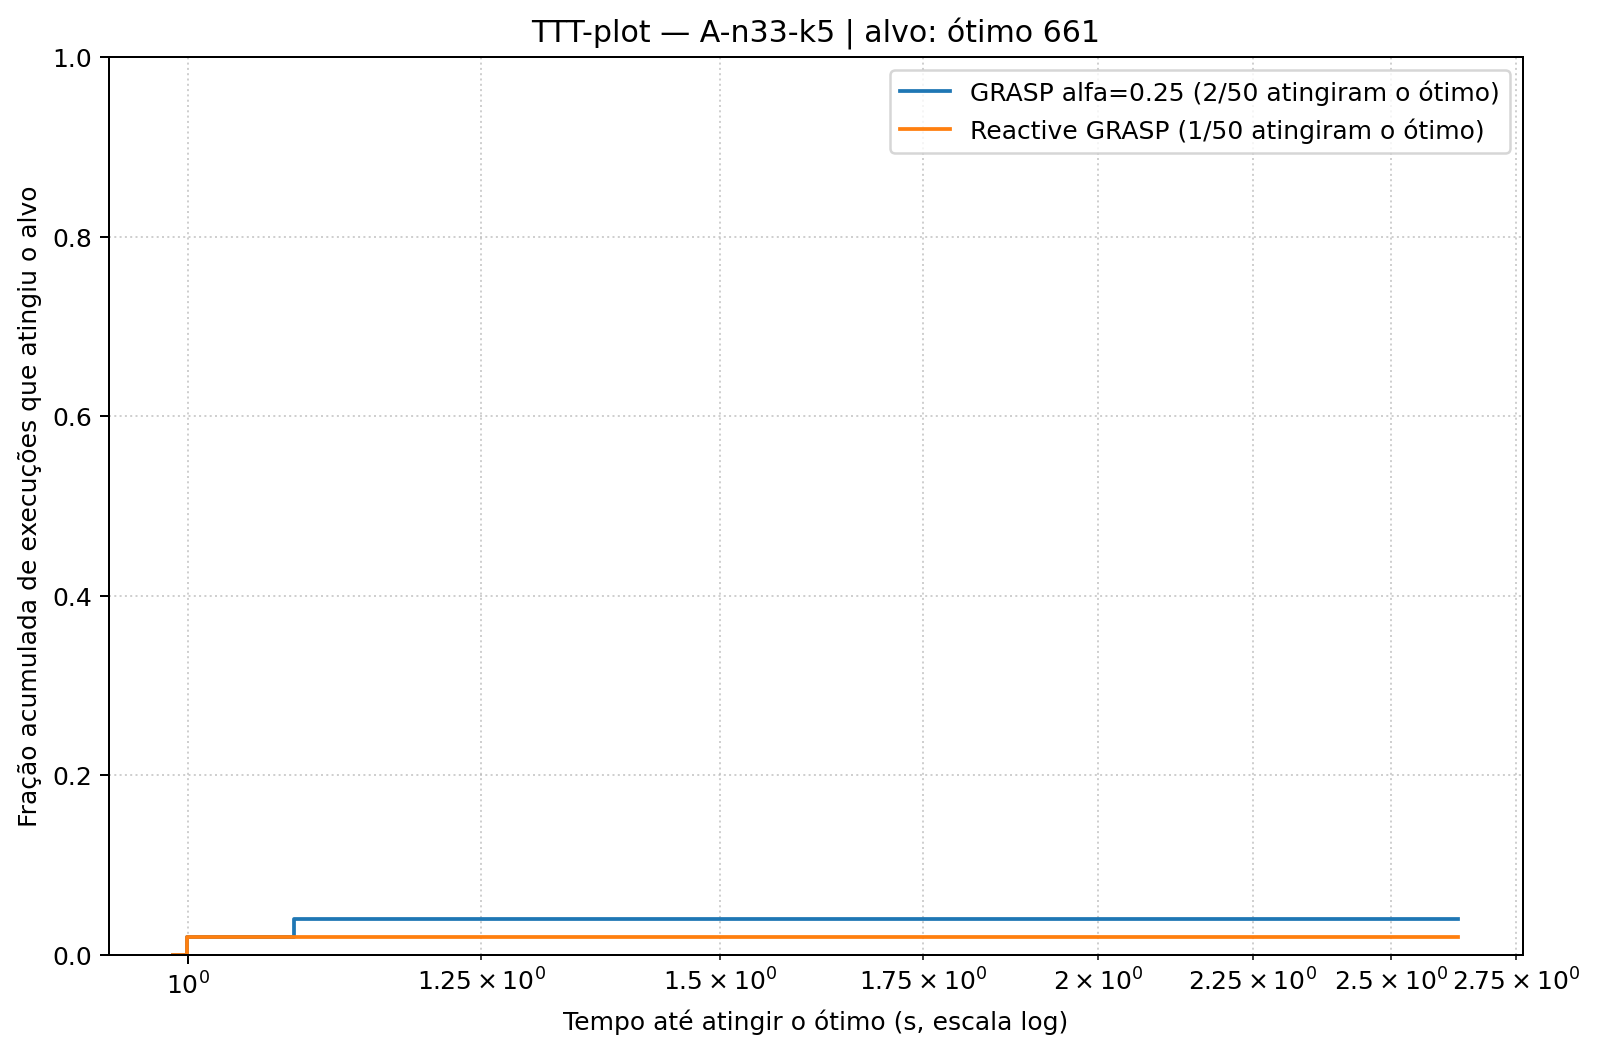
\includegraphics[width=0.98\textwidth]{imagens/ttt_A-n33-k5.png}
\caption{TTT em A-n33-k5.}
\label{fig:tttA}
\end{figure}

\begin{figure}[htbp]
\centering
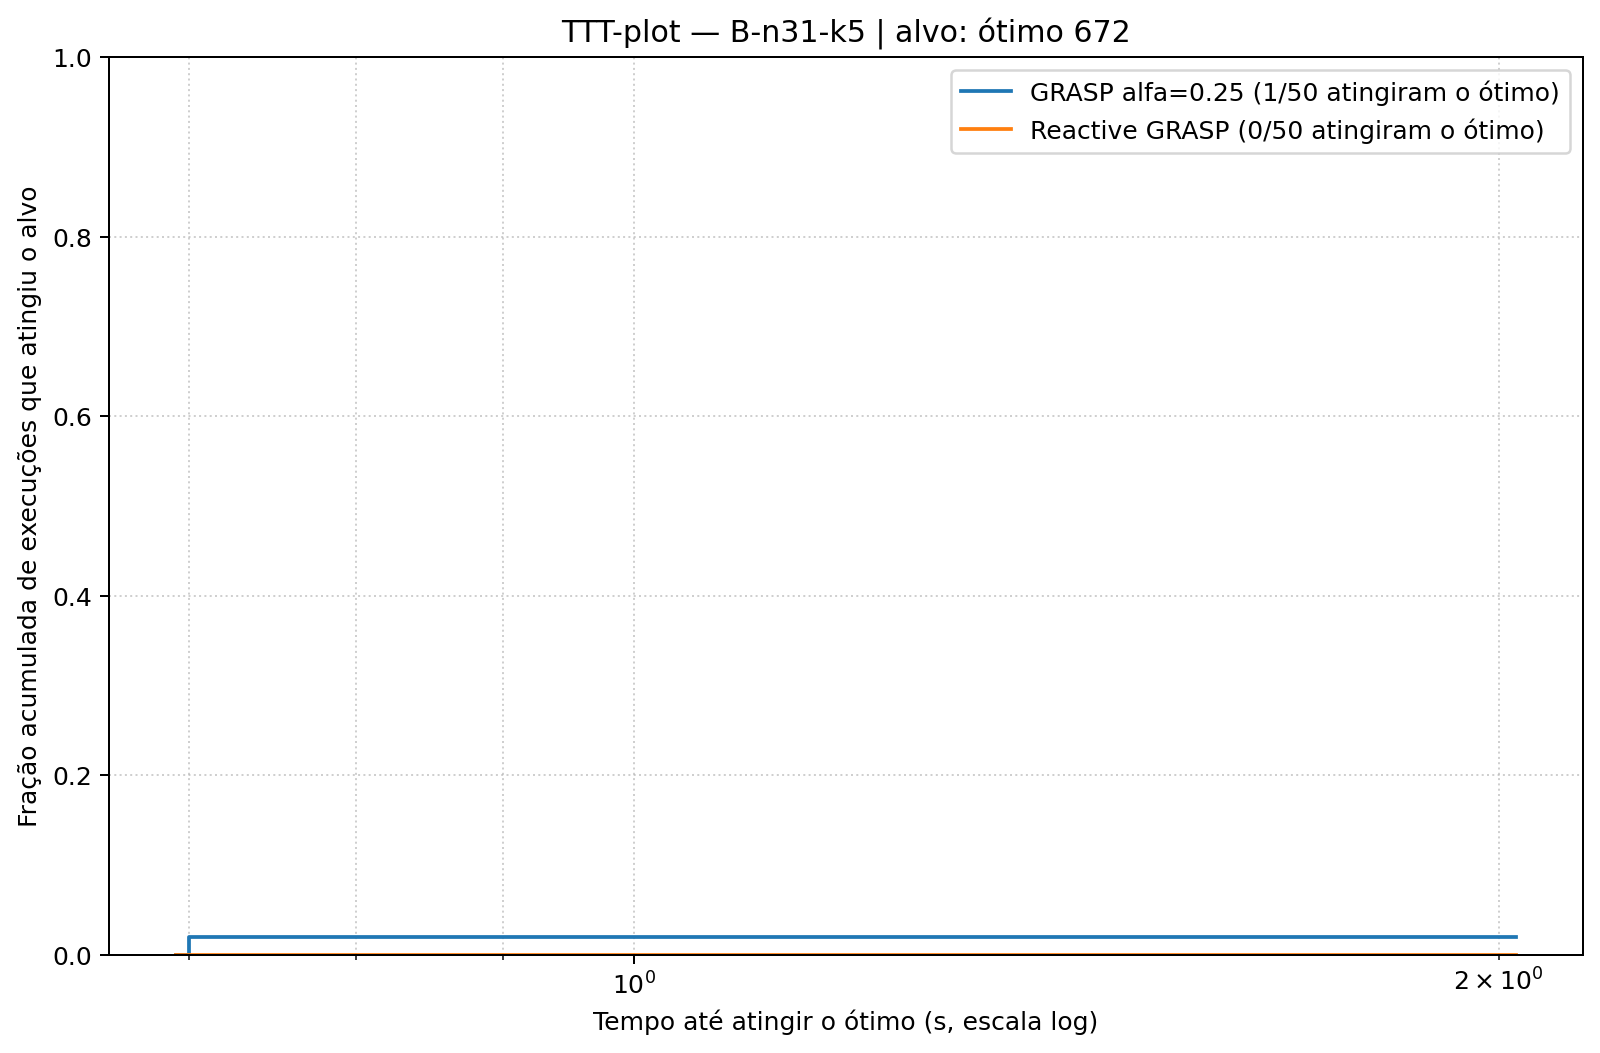
\includegraphics[width=0.98\textwidth]{imagens/ttt_B-n31-k5.png}
\caption{TTT em B-n31-k5.}
\label{fig:tttB}
\end{figure}

Em A-n33-k5, o tempo médio até o alvo foi cerca de 0.695 s no clássico e 0.280 s no reativo. Em B-n31-k5, somente o clássico encontrou o alvo, após cerca de 0.297 s. Como cada instância foi executada cinco vezes no experimento agregado, o mínimo representa o melhor resultado e a média representa a estabilidade observada.
